\documentclass[tikz,border=12pt]{standalone}
\usepackage{amsmath,amssymb}
\usetikzlibrary{calc,arrows.meta}

\begin{document}
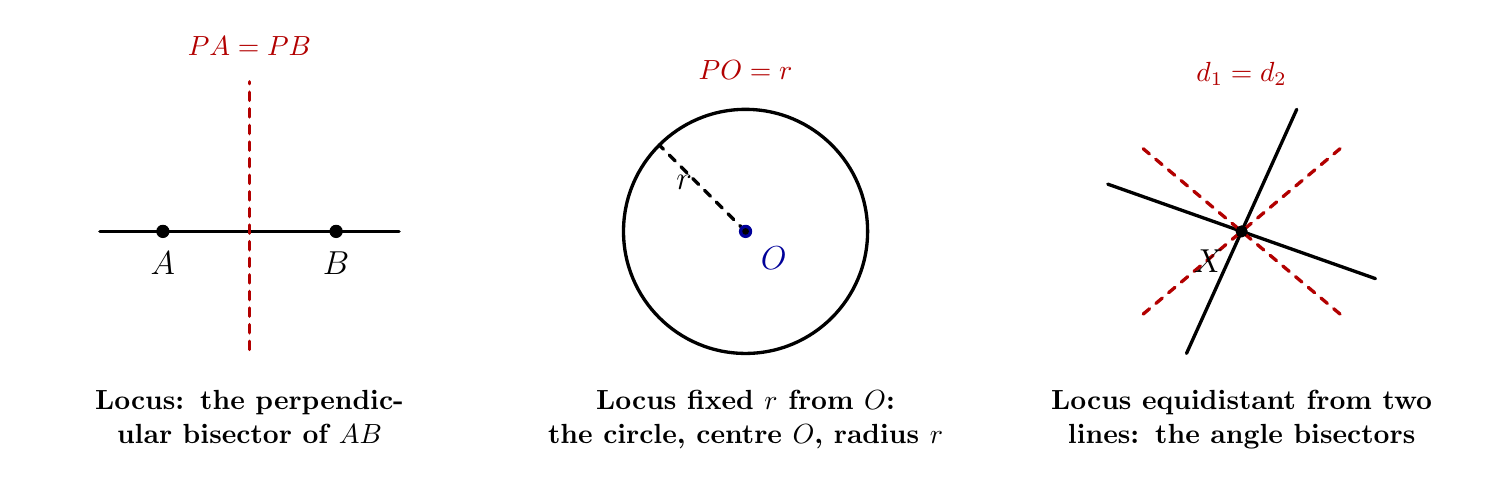
\begin{tikzpicture}[>=latex, line cap=round, line join=round]

  % =================== Board 1: two fixed points ===================
  \begin{scope}[shift={(0,0)}]
    \coordinate (A) at (-1.1,0);
    \coordinate (B) at (1.1,0);
    \draw[very thick] (-1.9,0) -- (1.9,0);
    \filldraw (A) circle (2.2pt) node[below=4pt, font=\large\bfseries] {$A$};
    \filldraw (B) circle (2.2pt) node[below=4pt, font=\large\bfseries] {$B$};
    \draw[very thick, red!70!black, dashed] (0,-1.5) -- (0,1.9);
    \node[red!70!black, font=\bfseries] at (0,2.35) {$PA = PB$};
    \node[font=\bfseries, anchor=north, align=center, text width=5.4cm] at (0,-1.9)
      {Locus: the perpendicular bisector of $AB$};
  \end{scope}

  % =================== Board 2: one fixed point ===================
  \begin{scope}[shift={(6.3,0)}]
    \coordinate (O) at (0,0);
    \draw[very thick] (0,0) circle (1.55);
    \draw[very thick, dashed] (0,0) -- (-1.1,1.1);
    \filldraw[blue!60!black] (O) circle (2.2pt) node[below right=2pt, font=\large\bfseries] {$O$};
    \filldraw (0,0) circle (1pt);
    \node[font=\large] at (-0.78,0.62) {$r$};
    \node[red!70!black, font=\bfseries] at (0,2.05) {$PO = r$};
    \node[font=\bfseries, anchor=north, align=center, text width=5.4cm] at (0,-1.9)
      {Locus fixed $r$ from $O$:\\ the circle, centre $O$, radius $r$};
  \end{scope}

  % =================== Board 3: two intersecting lines ===================
  \begin{scope}[shift={(12.6,0)}]
    \coordinate (X) at (0,0);
    \draw[very thick] (-1.7,0.6) -- (1.7,-0.6);
    \draw[very thick] (-0.7,-1.55) -- (0.7,1.55);
    % bisectors (dotted)
    \draw[very thick, red!70!black, dashed] (-1.25,-1.05) -- (1.25,1.05);
    \draw[very thick, red!70!black, dashed] (1.25,-1.05) -- (-1.25,1.05);
    \filldraw (X) circle (2pt) node[below left=3pt, font=\large\bfseries] {$X$};
    \node[red!70!black, font=\bfseries] at (0,2.0) {$d_1 = d_2$};
    \node[font=\bfseries, anchor=north, align=center, text width=5.4cm] at (0,-1.9)
      {Locus equidistant from two lines: the angle bisectors};
  \end{scope}

\end{tikzpicture}
\end{document}
